\chapter{Overview of Controls}
 
Since Cataclysm: Dark Days Ahead is an ASCII Game (a complex one at that), the control scheme is different from the modern day type of games. You will be required to utilize all of your keyboards' buttons to get every possible action done. Another factor is the capitalization of letters. so [e] is another Button altogether than [E].
 
Movement is done either by using the keyboard's numeric keyPad, with each of the buttons representing one of the 8 directions and [5] being the wait option. There is also the option of using a different control layout using the right side of the keyboard, yet this is probably more difficult to use.

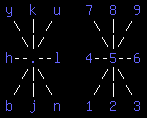
\includegraphics{01}

Buttons of interest:

[@] - character overview \newline
[i] - inventory screen \newline
[E] - consume an item from inventory or close by \newline
[a] - use an item from inventory or close by \newline
[A] - activate currently held item \newline
[d] - drop something \newline
[D] + directional input - drop something onto that location\newline
[e] + directional input - examine something that lies in the direction you gave input to. This allows for pickup from a location, like taking something from a freezer or oven and can open contextual menus (e.g. Curtains)\newline
[\%] - contextual menu - this is a comprehensive list of actions you can perform with the tools and items at hand.\newline
[x], [;] - Look around, this lets you freely move the camera around your field of view.\newline
[TAB] - auto-attack nearby enemies (including at range if you wield a weapon with reach)\newline
[X] + directional input - peek around that location, perfect for peeking around corners, as it will allow to see what is around without those actually notice you.\newline
[o] - open a door\newline
[c] - close a door\newline
[s] + directional input - smash something in that location\newline
[g], [,] - pick up items\newline
[G] - grab Item/Furniture - allows you to pull things along, like small vehicles, bookcases and the likes.\newline
[B] - butcher something you are standing on, also allows for disassembly if you meet the requirements.\newline
[V] - list everything around the player that is in sight. this can be toggled to monster view or item view using [TAB] and [s]-orted into either category or range to player\newline
[W] - wear item that is nearby or in your inventory\newline
[T] - take off a piece of clothing\newline
[w] - wield item nearby or in your inventory\newline
[R] - read something\newline
[r] - reload items that require ammunition\newline
[U] - unload item\newline
[t] - throw something\newline
[f] - fire held item\newline
[p] - open the Bionics' overview\newline
[\^{}] - control vehicle, if used on a tile that has no controls, allows for input to open the vehicles' control menu\newline
["] - toggle sprint/walk\newline
[\$] - go to sleep\newline
[\&] - crafting menu\newline
[*] - construction menu\newline
[\textbackslash] - haul items on the ground\newline
[/] - advanced inventory screen\newline
[[] - Open mutations screen - allows to activate/toggle eligible mutations
 
Remember - keys can be rebound and this is only a small selection for those that want to get a general idea of what does what. Consult the keybindings menu for a full overview of all the keys. 